% Soubory musí být v kódování, které je nastaveno v příkazu \usepackage[...]{inputenc}

\documentclass[%        Základní nastavení
%  draft,    				  % Testovací překlad
  12pt,       				% Velikost základního písma je 12 bodů
  a4paper,    				% Formát papíru je A4
  %oneside,      			% Jednostranný tisk
	twoside,      			% Dvoustranný tisk (kapitoly a další důležité části tedy začínají na lichých stranách)
	unicode,						% Záložky a metainformace ve výsledném  PDF budou v kódování unicode
]{report}				    	% Dokument třídy 'zpráva', vhodná pro sazbu závěrečných prací s kapitolami

\usepackage[utf8]		  %	Kódování zdrojových souborů je UTF-8
	{inputenc}					% Balíček pro nastavení kódování zdrojových souborů

\usepackage[				% Nastavení geometrie stránky
	bindingoffset=10mm,		% Hřbet pro vazbu
	hmargin={25mm,25mm},	% Vnitřní a vnější okraj  (jsou nehezky shodné; jakási úroveň estetiky je dosažena pomocí hřbetu)
	vmargin={25mm,34mm},	% Horní a dolní okraj
	footskip=17mm,			  % Velikost zápatí
	nohead,					      % Bez záhlaví
	marginparsep=2mm,		  % Vzdálenost marginálií
	marginparwidth=18mm,	% Šířka marginálií
]{geometry}

\usepackage{sectsty}
	%přetypuje nadpisy všech úrovní na bezpatkové, kromě \chapter, která je přenastavena zvlášť v thesis.sty
	\allsectionsfont{\sffamily}

\usepackage{graphicx} % Balíček 'graphicx' pro vkládání obrázků
											% Nutné pro vložení logotypů školy a fakulty

\usepackage[          % Balíček 'acronym' pro sazby zkratek a symbolů
	nohyperlinks				% Nebudou tvořeny hypertextové odkazy do seznamu zkratek
]{acronym}						
											% Nutné pro použití prostředí 'acronym' balíčku 'thesis'

\usepackage[
	breaklinks=true,		% Hypertextové odkazy mohou obsahovat zalomení řádku
	hypertexnames=false % Názvy hypertext. odkazů budou tvořeny nezávisle na názvech TeXu
]{hyperref}						% Balíček 'hyperref' pro sazbu hypertextových odkazů
											% Nutné pro použití příkazu 'pdfsettings' balíčku 'thesis'

\usepackage{pdfpages} % Balíček umožňující vkládat stránky z PDF souborů
                      % Nutné při vkládání titulních listů a zadání přímo
                      % ve formátu PDF z informačního systému

\usepackage{enumitem} % Balíček pro nastavení mezerování v odrážkách
  \setlist{topsep=0pt,partopsep=0pt,noitemsep} % konkrétní nastavení

\usepackage{cmap} 		% Balíček cmap zajišťuje, že PDF vytvořené `pdflatexem' je
											% plně "prohledávatelné" a "kopírovatelné"

%\usepackage{upgreek}	% Balíček pro sazbu stojatých řeckých písmem
											%% např. stojaté pí: \uppi
											%% např. stojaté mí: \upmu (použitelné třeba v mikrometrech)
											%% pozor, grafická nekompatibilita s fonty typu Computer Modern!
                      
%\usepackage{amsmath} %balíček pro sabu náročnější matematiky                 

\usepackage{dirtree}	% sazba adresářové struktury
                      % vhodné pro prezentaci obsahu elektronické přílohy (např. CD)

\usepackage[formats]{listings}	% Balíček pro sazbu zdrojových textů
\lstset{              % nastavení
%	Definice jazyka použitého ve výpisech
%    language=[LaTeX]{TeX},	% LaTeX
%	language={Matlab},		% Matlab
	language={C},           % jazyk C
    basicstyle=\ttfamily,	% definice základního stylu písma
    tabsize=2,			% definice velikosti tabulátoru
    inputencoding=utf8,         % pro soubory uložené v kódování UTF-8
		columns=fixed,  %fixed nebo flexible,
		fontadjust=true %licovani sloupcu
    extendedchars=true,
    literate=%  definice symbolů s diakritikou
    {á}{{\'a}}1
    {č}{{\v{c}}}1
    {ď}{{\v{d}}}1
    {é}{{\'e}}1
    {ě}{{\v{e}}}1
    {í}{{\'i}}1
    {ň}{{\v{n}}}1
    {ó}{{\'o}}1
    {ř}{{\v{r}}}1
    {š}{{\v{s}}}1
    {ť}{{\v{t}}}1
    {ú}{{\'u}}1
    {ů}{{\r{u}}}1
    {ý}{{\'y}}1
    {ž}{{\v{z}}}1
    {Á}{{\'A}}1
    {Č}{{\v{C}}}1
    {Ď}{{\v{D}}}1
    {É}{{\'E}}1
    {Ě}{{\v{E}}}1
    {Í}{{\'I}}1
    {Ň}{{\v{N}}}1
    {Ó}{{\'O}}1
    {Ř}{{\v{R}}}1
    {Š}{{\v{S}}}1
    {Ť}{{\v{T}}}1
    {Ú}{{\'U}}1
    {Ů}{{\r{U}}}1
    {Ý}{{\'Y}}1
    {Ž}{{\v{Z}}}1
}

%%%%%%%%%%%%%%%%%%%%%%%%%%%%%%%%%%%%%%%%%%%%%%%%%%%%%%%%%%%%%%%%%
%%%%%%      Definice informací o dokumentu             %%%%%%%%%%
%%%%%%%%%%%%%%%%%%%%%%%%%%%%%%%%%%%%%%%%%%%%%%%%%%%%%%%%%%%%%%%%%

% V tomto souboru se nastavují téměř veškeré informace, proměnné mezi studenty:
% jméno, název práce, pohlaví atd.
% Tento soubor je SDÍLENÝ mezi textem práce a prezentací k obhajobě -- netřeba něco nastavovat na dvou místech.

\usepackage[
%%% Z následujících voleb jazyka lze použít pouze jednu
  czech-english,		% originální jazyk je čeština, překlad je anglicky (výchozí)
  %english-czech,	% originální jazyk je angličtina, překlad je česky
  %slovak-english,	% originální jazyk je slovenština, překlad je anglicky
  %english-slovak,	% originální jazyk je angličtina, překlad je slovensky
%
%%% Z následujících voleb typu práce lze použít pouze jednu
  semestral,		  % semestrální práce (výchozí)
  %bachelor,			%	bakalářská práce
  %master,			  % diplomová práce
  %treatise,			% pojednání o disertační práci
  %doctoral,			% disertační práce
%
%%% Z následujících voleb zarovnání objektů lze použít pouze jednu
%  left,				  % rovnice a popisky plovoucích objektů budou zarovnány vlevo
	center,			    % rovnice a popisky plovoucích objektů budou zarovnány na střed (vychozi)
%
]{thesis}   % Balíček pro sazbu studentských prací


%%% Jméno a příjmení autora ve tvaru
%  [tituly před jménem]{Křestní}{Příjmení}[tituly za jménem]
% Pokud osoba nemá titul před/za jménem, smažte celý řetězec '[...]'
\author[]{Jakub}{Charvot}

%%% Identifikační číslo autora (VUT ID)
\butid{240844}

%%% Pohlaví autora/autorky
% (nepoužije se ve variantě english-czech ani english-slovak)
% Číselná hodnota: 1...žena, 0...muž
\gender{0}

%%% Jméno a příjmení vedoucího/školitele včetně titulů
%  [tituly před jménem]{Křestní}{Příjmení}[tituly za jménem]
% Pokud osoba nemá titul před/za jménem, smažte celý řetězec '[...]'
\advisor[Ing.]{Pavel}{Tomíček}[]

%%% Jméno a příjmení oponenta včetně titulů
%  [tituly před jménem]{Křestní}{Příjmení}[tituly za jménem]
% Pokud osoba nemá titul před/za jménem, smažte celý řetězec '[...]'
% Nastavení oponenta se uplatní pouze v prezentaci k obhajobě;
% v případě, že nechcete, aby se na titulním snímku prezentace zobrazoval oponent, pouze příkaz zakomentujte;
% u obhajoby semestrální práce se oponent nezobrazuje (jelikož neexistuje)
% U dizertační práce jsou typicky dva až tři oponenti. Pokud je chcete mít na titulním slajdu, prosím ručně odkomentujte a upravte jejich jména v definici "VUT title page" v souboru thesis.sty.
\opponent[doc.]{Oponent}{Krutý}[Ph.D.]

%%% Název práce
%  Parametr ve složených závorkách {} je název v originálním jazyce,
%  parametr v hranatých závorkách [] je překlad (podle toho jaký je originální jazyk).
%  V případě, že název Vaší práce je dlouhý a nevleze se celý do zápatí prezentace, použijte příkaz
%  \def\insertshorttitle{Zkác.\ náz.\ práce}
%  kde jako parametr vyplníte zkrácený název. Pokud nechcete zkracovat název, budete muset předefinovat,
%  jak se vytváří patička slidu. Viz odkaz: https://bit.ly/3EJTp5A
\title[Autonomous aquarium]{Autonomní akvárium}

%%% Označení oboru studia
%  Parametr ve složených závorkách {} je název oboru v originálním jazyce,
%  parametr v hranatých závorkách [] je překlad
\specialization[Microelectronics and Technology]{Mikroelektronika a technologie}

%%% Označení ústavu
%  Parametr ve složených závorkách {} je název ústavu v originálním jazyce,
%  parametr v hranatých závorkách [] je překlad
%\department[Department of Control and Instrumentation]{Ústav automatizace a měřicí techniky}
%\department[Department of Biomedical Engineering]{Ústav biomedicínského inženýrství}
%\department[Department of Electrical Power Engineering]{Ústav elektroenergetiky}
%\department[Department of Electrical and Electronic Technology]{Ústav elektrotechnologie}
%\department[Department of Physics]{Ústav fyziky}
%\department[Department of Foreign Languages]{Ústav jazyků}
%\department[Department of Mathematics]{Ústav matematiky}
\department[Department of Microelectronics]{Ústav mikroelektroniky}
%\department[Department of Radio Electronics]{Ústav radioelektroniky}
%\department[Department of Theoretical and Experimental Electrical Engineering]{Ústav teoretické a experimentální elektrotechniky}
% \department[Department of Telecommunications]{Ústav telekomunikací}
%\department[Department of Power Electrical and Electronic Engineering]{Ústav výkonové elektrotechniky a elektroniky}

%%% Označení fakulty
%  Parametr ve složených závorkách {} je název fakulty v originálním jazyce,
%  parametr v hranatých závorkách [] je překlad
%\faculty[Faculty of Architecture]{Fakulta architektury}
\faculty[Faculty of Electrical Engineering and~Communication]{Fakulta elektrotechniky a~komunikačních technologií}
%\faculty[Faculty of Chemistry]{Fakulta chemická}
%\faculty[Faculty of Information Technology]{Fakulta informačních technologií}
%\faculty[Faculty of Business and Management]{Fakulta podnikatelská}
%\faculty[Faculty of Civil Engineering]{Fakulta stavební}
%\faculty[Faculty of Mechanical Engineering]{Fakulta strojního inženýrství}
%\faculty[Faculty of Fine Arts]{Fakulta výtvarných umění}
%
%Nastavení logotypu (v hranatych zavorkach zkracene logo, ve slozenych plne):
\facultylogo[logo/FEKT_zkratka_barevne_PANTONE_CZ]{logo/UTKO_color_PANTONE_CZ}

%%% Rok odevzdání práce
\graduateyear{2024}
%%% Akademický rok odevzdání práce
\academicyear{2023/24}

%%% Datum obhajoby (uplatní se pouze v prezentaci k obhajobě)
\date{11.\,11.\,1980} 

%%% Místo obhajoby
% Na titulních stránkách bude automaticky vysázeno VELKÝMI písmeny (pokud tyto stránky sází šablona)
\city{Brno}

%%% Abstrakt
\abstract[%
This thesis delves into the topic of~aquarium automation, aiming to~design custom device for this purpose. A~market survey is~presented with depiction of~existing commercial solutions in~the~field of~automation, also the~essential technology requirements for~efficient aquarium operation are summarized. Regarding the~design of~the~custom device, the~thesis explain the~chosen architecture and takes a~deeper look at~some of~its~parts. The main outcome of~this thesis is the~creation of~an~electrical schematic for the~control unit. The~present work will be followed by a bachelor's thesis, within which the~device will be completed.
]{%
Tato práce se zaměřuje na problematiku automatizace akvárií a jejím cílem je navrhnout vlastní zařízení sloužící tomuto účelu. V práci je proveden trůzkum trhu a popsána již existující komerční řešení věnující se právě automatizaci, také je zde obsaženo shrnutí minimální techniky potřebné pro provoz akvária. Z hlediska návrhu vlastního zařízení je obsažen popis a odůvodnění zvolené architektury, dále se text detailněji věnuje některým dílčím blokům. Výstupem práce je zejména navržené elektrické schéma řídící jednotky. Na tuto práci bude navazovat bakalářská práce, v rámci které bude zařízení dokončeno. 
}

%%% Klíčová slova
\keywrds[%
aquaristics, automation, ESP32, data buses, device design
]{%
akvaristika, automatizace, ESP32, sběrnice, návrh zařízení
}


%%% Poděkování
\acknowledgement{%
Rád bych poděkoval vedoucímu semestrální práce
panu Ing.~Pavlu Tomíčkovi\ za ochotu i trpělivost, kterou se mnou měl po celou dobu tvorby této práce, a za mnoho cenných a podnětných rad k její odborné i formální stránce. Dále děkuji svému kamarádovi Radku Jančičkovi za osvětu v oblasti akvaristiky. 

}%  % do tohoto souboru doplňte údaje o sobě, druhu práce, názvu...

%%%%%%%%%%%%%%%%%%%%%%%%%%%%%%%%%%%%%%%%%%%%%%%%%%%%%%%%%%%%%%%%%%%%%%%%

%%%%%%%%%%%%%%%%%%%%%%%%%%%%%%%%%%%%%%%%%%%%%%%%%%%%%%%%%%%%%%%%%%%%%%%%
%%%%%%     Nastavení polí ve Vlastnostech dokumentu PDF      %%%%%%%%%%%
%%%%%%%%%%%%%%%%%%%%%%%%%%%%%%%%%%%%%%%%%%%%%%%%%%%%%%%%%%%%%%%%%%%%%%%%
%% Při načteném balíčku 'hyperref' lze použít příkaz '\pdfsettings':
\pdfsettings
%  Nastavení polí je možné provést také ručně příkazem:
%\hypersetup{
%  pdftitle={Název studentské práce},    	% Pole 'Document Title'
%  pdfauthor={Autor studenstké práce},   	% Pole 'Author'
%  pdfsubject={Typ práce}, 						  	% Pole 'Subject'
%  pdfkeywords={Klíčová slova}           	% Pole 'Keywords'
%}
%%%%%%%%%%%%%%%%%%%%%%%%%%%%%%%%%%%%%%%%%%%%%%%%%%%%%%%%%%%%%%%%%%%%%%%

\pdfmapfile{=vafle.map}

%%%%%%%%%%%%%%%%%%%%%%%%%%%%%%%%%%%%%%%%%%%%%%%%%%%%%%%%%%%%%%%%%%%%%%%
%%%%%%%%%%%       Začátek dokumentu               %%%%%%%%%%%%%%%%%%%%%
%%%%%%%%%%%%%%%%%%%%%%%%%%%%%%%%%%%%%%%%%%%%%%%%%%%%%%%%%%%%%%%%%%%%%%%
\begin{document}
\pagestyle{empty} %vypnutí číslování stránek

%%% Vložení desek -- od září 2021 na žádost fakulty nepoužíváno
%\includepdf[pages=1]%  buďto generovaných informačním systémem
  %{pdf/student-desky}% název souboru nesmí obsahovat mezery!
%%% NEBO vytvoření desek z balíčku
%%\makecover
%%%
%\oddpage % při dvojstranném tisku přidá prázdnou stránku
%% kazdopádně ale:
%\setcounter{page}{1} %resetovaní čítače stránek -- desky do číslování nezahrnujeme

%% Vložení titulního listu
\includepdf[pages=1]%    buďto generovaného informačním systémem
  {pdf/student-titulka}% název souboru nesmí obsahovat mezery!
%% NEBO vytvoření titulní stránky z balíčku
%\maketitle
%%
\oddpage  % při dvojstranném tisku se přidá prázdná stránka
   
%% Vložení zadání
\includepdf[pages=1]%   buďto generovaného informačním systémem
  {pdf/student-zadani}% název souboru nesmí obsahovat mezery!
%% NEBO lze vytvořit prázdný list příkazem ze šablony
%\patternpage{}%
%	{\sffamily\Huge\centering ZDE VLOŽIT LIST ZADÁNÍ}%
%	{\sffamily\centering Z~důvodu správného číslování stránek}
%%
\oddpage% při dvojstranném tisku se přidá prázdná stránka

%% Vysázení stránky s abstraktem
\makeabstract

% Vysázení stránky s rozšířeným abstraktem
% (pokud píšete práci v češtině či slovenštině, vložení rozšířeného abstraktu zrušte;
%  pro semestrální projekt také není potřeba rozšířený abstrakt uvádět)
% Vysázení stránky s rozšířeným abstraktem
% (týká se pouze bc. a dp. prací psaných v angličtině, viz Směrnice rektora 72/2017)
\cleardoublepage
\noindent
{\large\sffamily\bfseries\MakeUppercase{Rozšířený abstrakt}}
\\
Výtah ze směrnice rektora 72/2017:\\
\emph{Bakalářská a diplomová práce předložená v angličtině musí obsahovat rozšířený abstrakt v češtině
nebo slovenštině (čl. 15). To se netýká studentů, kteří studují studijní program akreditovaný v
angličtině.}
(čl. 3, par. 7)\\
\emph{Nebude-li vnitřní normou stanoveno jinak, doporučuje se rozšířený abstrakt o rozsahu přibližně 3
normostrany, který bude obsahovat úvod, popis řešení a shrnutí a~zhodnocení výsledků.}
(čl. 15, par. 5)

%%% Vysázení citace práce
\makecitation

%%% Vysázení prohlášení o samostatnosti
\makedeclaration

%%% Vysázení poděkování
\makeacknowledgement

%%% Vysázení obsahu
\tableofcontents

%%% Vysázení seznamu obrázků
% (vynechejte, pokud máte dva nebo méně obrázků)
\listoffigures

%%% Vysázení seznamu tabulek
% (vynechejte, pokud máte dvě nebo méně tabulek)
\listoftables

%%% Vysázení seznamu výpisů kódu
% (vynechejte, pokud máte dva nebo méně výpisů)
\lstlistoflistings

\cleardoublepage\pagestyle{plain}   % zapnutí číslování stránek

%Pro vkládání kapitol i příloh používejte raději \include než \input
%%% Vložení souboru 'text/uvod.tex' s úvodem
\chapter*{Úvod}
\phantomsection
\addcontentsline{toc}{chapter}{Úvod}


V dnešní době, kdy jsou na vzestupu fenomény jako chytrá domácnost, \acs{iot} (\acl{iot}) nebo Průmysl 4.0, se na trhu objevuje stále více výrobků, které se snaží automatizovat a zjednodušit různé oblasti našeho života. Tento trend se dnes dotýká nejedné volnočasové aktivity a to včetně akvaristiky. Tu lze samozřejmě provozovat na různé úrovni, ale i majitelé malých domácích akvárií potřebují k provozu svého koníčku relativně velké množství elektroniky. 
Běžnou praxí je, že každé z použitých zařízení je ovládáno buďto zcela ručně nebo, pokud disponuje možností vzdáleného přístupu a automatizace, má svou samostanou aplikaci a uživatel tak provoz akvária musí ovládat z několika různých míst, což může být značně nepohodlné a nepřehledné.

Na trhu samozřejmě existují také velmi sofistikované a komplexní systémy, ty ovšem svou cenou vysoce přesahují rozpočet běžného "domácího" akvaristy. Tato práce se věnuje návrhu a tvorbě zařízení, které má za cíl nabídnout pohodlnou kontrolu a ovládání všech potřebných součástí domácího akvária, a to při zachování jednoduchosti a nízké pořizovací ceny.

% \input{text/images/CMOS_images.tex}

%%% Vložení souboru 'text/cile.tex' s úvodem
\chapter*{Cíle práce}
\phantomsection
\addcontentsline{toc}{chapter}{Cíle práce}

Má tato kapitola existovat a nebo mám cíle podrobněji rozebrat v~úvodu? 

%%% Vložení souboru 'text/reseni' s popisem řešení práce
% (rozdělte na více souborů či kapitol, pokud je vhodné)
\chapter{Teoretická část studentské práce}

Teoretické zázemí studentské práce vhodně rozdělené do částí.

(Struktura navržená v~této šabloně je nejhrubší možná, po konzultaci s~vedoucím je vhodné zvolit přiléhavější.)


%%% Vložení souboru 'text/vysledky' s popisem vysledků práce
% (rozdělte na více souborů či kapitol, pokud je vhodné)
\chapter{Výsledky studentské práce}

Praktická část a výsledky studentské práce vhodně rozdělené do částí.

\section{Programové řešení}
Lorem ipsum dolor sit amet, consectetuer adipiscing elit. Nulla pulvinar eleifend sem. Integer in sapien. Etiam sapien elit, consequat eget, tristique non, venenatis quis, ante. In laoreet, magna id viverra tincidunt, sem odio bibendum justo, vel imperdiet sapien wisi sed libero. Phasellus enim erat, vestibulum vel, aliquam a, posuere eu, velit. Aliquam erat volutpat. Nullam faucibus mi quis velit \cite{sr72/2017}.

\section{Výsledky měření}
Fusce tellus odio, dapibus id fermentum quis, suscipit id erat. Fusce tellus. Morbi scelerisque luctus velit. In laoreet, magna id viverra tincidunt, sem odio bibendum justo, vel imperdiet sapien wisi sed libero. Quisque porta. Fusce suscipit libero eget elit. Nulla non lectus sed nisl molestie malesuada. Phasellus faucibus molestie nisl. Integer vulputate sem a nibh rutrum consequat. Proin mattis lacinia justo. Phasellus et lorem id felis nonummy placerat. Etiam ligula pede, sagittis quis, interdum ultricies, scelerisque eu. Cras elementum. Aenean placerat. Donec ipsum massa, ullamcorper in, auctor et, scelerisque sed, est. Aliquam ante. Integer imperdiet lectus quis justo. Vivamus ac leo pretium faucibus. Nullam faucibus mi quis velit.

\subsection{Etiam quis quam}
Neque porro quisquam est, qui dolorem ipsum quia dolor sit amet, consectetur, adipisci velit, sed quia non numquam eius modi tempora incidunt ut labore et dolore magnam aliquam quaerat voluptatem. Aliquam erat volutpat. Lorem ipsum dolor sit amet, consectetuer adipiscing elit \cite{sr72/2017,pravidla}. Nunc auctor. Neque porro quisquam est, qui dolorem ipsum quia dolor sit amet, consectetur, adipisci velit, sed quia non numquam eius modi tempora incidunt ut labore et dolore magnam aliquam quaerat voluptatem. Maecenas lorem. Maecenas libero. In laoreet, magna id viverra tincidunt, sem odio bibendum justo, vel imperdiet sapien wisi sed libero. Nullam rhoncus aliquam metus.

\subsubsection{Integer rutrum orci vestibulum}
Integer rutrum, orci vestibulum ullamcorper ultricies, lacus quam ultricies odio, vitae placerat pede sem sit amet enim. Ut enim ad minim veniam, quis nostrud exercitation ullamco laboris nisi ut aliquip ex ea commodo consequat. Fusce tellus odio, dapibus id fermentum quis, suscipit id erat. Nullam eget nisl. Nunc auctor. Etiam dui sem, fermentum vitae, sagittis id, malesuada in, quam. Fusce dui leo, imperdiet in, aliquam sit amet, feugiat eu, orci. Curabitur vitae diam non enim vestibulum interdum. Aliquam erat volutpat. Pellentesque sapien. Phasellus enim erat, vestibulum vel, aliquam a, posuere eu, velit.

\subsubsection{Eger rutrum orci westibulum}
Fusce dui leo, imperdiet in, aliquam sit amet, feugiat eu, orci. Maecenas aliquet accumsan leo. Aliquam ornare wisi eu metus. Cum sociis natoque penatibus et magnis dis parturient montes, nascetur ridiculus mus. Aliquam erat volutpat. Donec iaculis gravida nulla. Sed elit dui, pellentesque a, faucibus vel, interdum nec, diam. Temporibus autem quibusdam et aut officiis debitis aut rerum necessitatibus saepe eveniet ut et voluptates repudiandae sint et molestiae non recusandae. Nulla non arcu lacinia neque faucibus fringilla. Phasellus enim erat, vestibulum vel, aliquam a, posuere eu, velit. Praesent vitae arcu tempor neque lacinia pretium
\cite{Walter1999,Svacina1999IEEE,RajmicSysel2002}.

Aliquam erat volutpat. Quisque porta. Integer imperdiet lectus quis justo. Nullam justo enim, consectetuer nec, ullamcorper ac, vestibulum in, elit. Nullam faucibus mi quis velit. Fusce tellus. Fusce consectetuer risus a nunc. Cras pede libero, dapibus nec, pretium sit amet, tempor quis. Morbi imperdiet, mauris ac auctor dictum, nisl ligula egestas nulla, et sollicitudin sem purus in lacus
\cite{CSN_ISO_690-2022,CSN_ISO_7144-1997,CSN_ISO_31-11}.
Mauris elementum mauris vitae tortor. Neque porro quisquam est, qui dolorem ipsum quia dolor sit amet, consectetur, adipisci velit, sed quia non numquam eius modi tempora incidunt ut labore et dolore magnam aliquam quaerat voluptatem. Quisque porta. Integer vulputate sem a nibh rutrum consequat. Nulla pulvinar eleifend sem. Praesent id justo in neque elementum ultrices \cite{Farkasova23:CSNISO6902022komentar}.

Fusce suscipit libero eget elit. Integer vulputate sem a nibh rutrum consequat. Aliquam erat volutpat. Etiam neque. Nulla turpis magna, cursus sit amet, suscipit a, interdum id, felis. Nullam rhoncus aliquam metus. Etiam dui sem, fermentum vitae, sagittis id, malesuada in, quam. Nunc auctor. Nunc dapibus tortor vel mi dapibus sollicitudin. Praesent in mauris eu tortor porttitor accumsan. Nulla non arcu lacinia neque faucibus fringilla. Nullam lectus justo, vulputate eget mollis sed, tempor sed magna. Maecenas lorem. Aenean placerat. Donec vitae arcu. Maecenas lorem. Donec iaculis gravida nulla. Nulla non lectus sed nisl molestie malesuada.

Duis pulvinar. Nulla est. Duis condimentum augue id magna semper rutrum. Integer pellentesque quam vel velit. Aliquam ante. Nulla quis diam. Proin mattis lacinia justo. Aenean fermentum risus id tortor. Nunc auctor. Nullam justo enim, consectetuer nec, ullamcorper ac, vestibulum in, elit. In dapibus augue non sapien. Etiam bibendum elit eget erat. In sem justo, commodo ut, suscipit at, pharetra vitae, orci. Maecenas libero.

Nulla non lectus sed nisl molestie malesuada. Donec vitae arcu. Aenean fermentum risus id tortor. Praesent in mauris eu tortor porttitor accumsan. Nulla pulvinar eleifend sem. Duis viverra diam non justo. Integer imperdiet lectus quis justo. Pellentesque habitant morbi tristique senectus et netus et malesuada fames ac turpis egestas. In rutrum. Excepteur sint occaecat cupidatat non proident, sunt in culpa qui officia deserunt mollit anim id est laborum. Nulla non lectus sed nisl molestie malesuada. Aliquam erat volutpat. Mauris tincidunt sem sed arcu. Duis bibendum, lectus ut viverra rhoncus, dolor nunc faucibus libero, eget facilisis enim ipsum id lacus. Fusce tellus odio, dapibus id fermentum quis, suscipit id erat. In enim a arcu imperdiet malesuada. Nulla non lectus sed nisl molestie malesuada. Proin mattis lacinia justo.

Aliquam in lorem sit amet leo accumsan lacinia. Cum sociis natoque penatibus et magnis dis parturient montes, nascetur ridiculus mus. Duis sapien nunc, commodo et, interdum suscipit, sollicitudin et, dolor. Suspendisse sagittis ultrices augue. Nullam lectus justo, vulputate eget mollis sed, tempor sed magna. In convallis. Praesent id justo in neque elementum ultrices. Neque porro quisquam est, qui dolorem ipsum quia dolor sit amet, consectetur, adipisci velit, sed quia non numquam eius modi tempora incidunt ut labore et dolore magnam aliquam quaerat voluptatem.

Pellentesque pretium lectus id turpis. Nemo enim ipsam voluptatem quia voluptas sit aspernatur aut odit aut fugit, sed quia consequuntur magni dolores eos qui ratione voluptatem sequi nesciunt. Curabitur ligula sapien, pulvinar a vestibulum quis, facilisis vel sapien. Praesent dapibus. Sed elit dui, pellentesque a, faucibus vel, interdum nec, diam. Duis viverra diam non justo. Duis ante orci, molestie vitae vehicula venenatis, tincidunt ac pede. Phasellus rhoncus. Maecenas fermentum, sem in pharetra pellentesque, velit turpis volutpat ante, in pharetra metus odio a lectus. Proin pede metus, vulputate nec, fermentum fringilla, vehicula vitae, justo. Fusce aliquam vestibulum ipsum. Nullam at arcu a est sollicitudin euismod.

%Aliquam ante. Phasellus faucibus molestie nisl. Etiam ligula pede, sagittis quis, interdum ultricies, scelerisque eu. Morbi leo mi, nonummy eget tristique non, rhoncus non leo. Cum sociis natoque penatibus et magnis dis parturient montes, nascetur ridiculus mus. Morbi scelerisque luctus velit. Curabitur bibendum justo non orci. Donec quis nibh at felis congue commodo. Nullam faucibus mi quis velit. Aenean id metus id velit ullamcorper pulvinar. Pellentesque sapien. Fusce nibh. Vestibulum fermentum tortor id mi. Nullam eget nisl. Praesent vitae arcu tempor neque lacinia pretium. Proin in tellus sit amet nibh dignissim sagittis. Donec quis nibh at felis congue commodo.
%
%Nam quis nulla. Proin in tellus sit amet nibh dignissim sagittis. Nullam dapibus fermentum ipsum. Curabitur ligula sapien, pulvinar a vestibulum quis, facilisis vel sapien. Nam libero tempore, cum soluta nobis est eligendi optio cumque nihil impedit quo minus id quod maxime placeat facere possimus, omnis voluptas assumenda est, omnis dolor repellendus. Vivamus ac leo pretium faucibus. Nunc tincidunt ante vitae massa. Maecenas sollicitudin. Ut tempus purus at lorem. Nullam lectus justo, vulputate eget mollis sed, tempor sed magna. Fusce consectetuer risus a nunc. Etiam quis quam.
%
%Donec quis nibh at felis congue commodo. Sed vel lectus. Donec odio tempus molestie, porttitor ut, iaculis quis, sem. Nullam feugiat, turpis at pulvinar vulputate, erat libero tristique tellus, nec bibendum odio risus sit amet ante. Sed elit dui, pellentesque a, faucibus vel, interdum nec, diam. Cras elementum. Sed vel lectus. Donec odio tempus molestie, porttitor ut, iaculis quis, sem. Etiam neque. Integer tempor. Vivamus porttitor turpis ac leo. Nulla non arcu lacinia neque faucibus fringilla.
%
%Etiam posuere lacus quis dolor. Nemo enim ipsam voluptatem quia voluptas sit aspernatur aut odit aut fugit, sed quia consequuntur magni dolores eos qui ratione voluptatem sequi nesciunt. Nullam faucibus mi quis velit. Cum sociis natoque penatibus et magnis dis parturient montes, nascetur ridiculus mus. Phasellus faucibus molestie nisl. Maecenas ipsum velit, consectetuer eu lobortis ut, dictum at dui. Maecenas aliquet accumsan leo. Pellentesque ipsum. Donec vitae arcu. Suspendisse nisl. Morbi imperdiet, mauris ac auctor dictum, nisl ligula egestas nulla, et sollicitudin sem purus in lacus. Pellentesque ipsum. Ut enim ad minima veniam, quis nostrum exercitationem ullam corporis suscipit laboriosam, nisi ut aliquid ex ea commodi consequatur? Nam libero tempore, cum soluta nobis est eligendi optio cumque nihil impedit quo minus id quod maxime placeat facere possimus, omnis voluptas assumenda est, omnis dolor repellendus.


%%% Vložení souboru 'text/zaver' se závěrem
\chapter*{Závěr}
\phantomsection
\addcontentsline{toc}{chapter}{Závěr}

V~rámci bakalářské práce bylo navrženo a sestaveno zařízení, určené k~ovládání běžného domácího akvária. Jedná se o~modulární systém sestávající z~řídicí jednotky a několika propojených modulů, které vzájemně komunikují po sběrnici CAN. K~systému byla také vytvořena jednoduchá webová stránka, přes kterou je možné systém vzdáleně konfigurovat a monitorovat. 

Teoretická část práce se věnuje problematice provozu akvária. Jsou zde rozebrány důležité veličiny, které je potřeba monitorovat a ovládat pro spolehlivé přežití akvarijního ekosystému. Dále se text věnuje průzkumu trhu a používané akvarijní technice. Postupováno je od nezbytného minima pro založení malého akvária, až po systémy zajišťující komplexní automatizaci velkých instalací, složených z~více nádrží.

Na základě provedené rešerše jsou stanoveny požadavky na podobu a funkci vlastního zařízení. Jeho cílem není konkurovat svými možnostmi drahým pokročilým systémům, ale spíše dosáhnout jistého kompromisu mezi cenou a stále dostatečně širokou funkcionalitou k~automatizaci menšího domácího akvária. Samotný návrh systému začíná popisem zvolené architektury, poté jsou podrobněji popsány jednotlivé dílčí části. Byly navrženy tři desky plošných spojů. Řídící jednotka obsahuje spínaný zdroj použitý k~napájení celého systému a mikrokontrolér ESP32 zajišťující kromě samotného řízení také komunikaci skrze síť WiFi. Moduly periferií jsou navrženy jako univerzální platforma, ke které lze připojit různé obvody sensorů nebo akčních členů. Pro plynulé ovládání LED osvětlení byla navržena vlastní deska, kterou lze do této platformy vložit. Ostatní periferie již nebyly tak komplexní a pro připojení sensorů k~univerzální platformě postačila prototypová deska. 

Zvolený způsob komunikace periferií a ovládání přes internet učinil systém velmi komplexní a proto při tvorbě softwaru vznikla řada překážek, kterým bylo potřeba čelit. Klíčové softwarové bloky byly zvládnuty úspěšně. Jednotlivé části systému mezi sebou vzájemně komunikují a možná je i konfigurace systému přes webové rozhraní, ta je navíc zachována v~paměti flash i po restartu zařízení. Stejně tak je zařízení schopné odesílat naměřená data, která si uživatel může na webu zobrazit. Samotný algoritmus řízení akvária ale zatím není dostačující k~úplnému a spolehlivému provozu a řadu funkcí bude potřeba dokončit. 

Jednotlivé dílčí části zařízení byly testovány postupně, z~důvodu nalezených chyb bude dlouhodobý test v~provozu akvária teprve následovat. 

Volba modulární architektury sice návrh zařízení značně zkomplikovala a díky tomuto rozhodnutí nebylo dosaženo všech vytyčených cílů, na druhou stranu je ale zařízení velmi flexibilní a do budoucna má potenciál sloužit nejen jako systém řízení akvária. S~drobným rozšířením může snadno obsloužit vícero oblastní domácí automatizace a stát se tak součástí moderního fenoménu tzv. Smart Home.

%%% Vložení souboru 'text/literatura' se seznamem zdrojů
% Pro sazbu seznamu literatury použijte jednu z následujících možností

%%%%%%%%%%%%%%%%%%%%%%%%%%%%%%%%%%%%%%%%%%%%%%%%%%%%%%%%%%%%%%%%%%%%%%%%%
%1) Seznam citací definovaný přímo pomocí prostředí literatura / thebibliography

% \begin{thebibliography}{99}
	
% \bibitem{sr72/2017}
% 	VYSOKÉ UČENÍ TECHNICKÉ V~BRNĚ.
% 	\emph{Směrnice č.\,72/2017, Úprava, odevzdávání a~zveřejňování závěrečných prací.}
% 	Online. Brno: VUT v~Brně, 2017.
% 	Úplné znění ke dni 11.\,4.\,2022.
% 	Dostupné z:\\
% 	{\small
% 	\url{https://www.vut.cz/uredni-deska/vnitrni-predpisy-a-dokumenty/smernice-c-72-2017-uprava-odevzdavani-a-zverejnovani-zaverecnych-praci-d161410}.}
% 	[cit.\ 2023-09-27].

% \bibitem{CSN_ISO_690-2022}
%     ÚŘAD PRO TECHNICKOU NORMALIZACI, METROLOGII A~STÁTNÍ ZKUŠEBNICTVÍ.
%     ČSN ISO 690:2022 (01 0197), \emph{Informace a dokumentace -- Pravidla pro bibliografické odkazy a~citace informačních zdrojů.}
%     Čtvrté vydání. Praha, 2022.

% \bibitem{CSN_ISO_7144-1997}
%     ÚŘAD PRO TECHNICKOU NORMALIZACI, METROLOGII A~STÁTNÍ ZKUŠEBNICTVÍ.
%     ČSN ISO 7144 (010161), \emph{Dokumentace -- Formální úprava disertací a~podobných dokumentů.}
% %    24 stran.
%     Praha, 1997.

% \bibitem{CSN_ISO_31-11}
%     ÚŘAD PRO TECHNICKOU NORMALIZACI, METROLOGII A~STÁTNÍ ZKUŠEBNICTVÍ.
%     ČSN ISO 31-11, \emph{Veličiny a~jednotky -- část 11: Matematické znaky a~značky používané ve fyzikálních vědách a~v~technice.}
%     Praha, 1999.

% \bibitem{Farkasova23:CSNISO6902022komentar}
% 	FARKAŠOVÁ, B. et al.
% 	\emph{Výklad normy ČSN ISO 690:2022 (01 0197) účinné od 1.\,12.\,2022}.
% 	 Online. První vydání. 2023.
% 	Dostupné~z:
% 	\url{https://www.citace.com/Vyklad-CSN-ISO-690-2022.pdf}.
% 	[cit.\,2023-09-27].

% \bibitem{pravidla}
%     \emph{Pravidla českého pravopisu}.
% 	1.\ vydání. Olomouc: FIN, 1998.\\
% 	\mbox{ISBN 80-86002-40-3}.

% \bibitem{Walter1999}
% 	WALTER, G.\,G. a SHEN, X.
% 	\emph{Wavelets and Other Orthogonal Systems}.
% 	2.\,vydání, Boca Raton: Chapman\,\&\,Hall/CRC, 2000.
% 	ISBN 1-58488-227-1

% \bibitem{Svacina1999IEEE}
% 	SVAČINA, J.
% 	Dispersion Characteristics of Multilayered Slotlines -- a Simple Approach.
% 	\emph{IEEE Transactions on Microwave Theory and Techniques}.
% 	1999, vol.\,47, no.\,9, s.\,1826--1829. ISSN 0018-9480.

% \bibitem{RajmicSysel2002}
%     RAJMIC, P. a SYSEL, P.
%     Wavelet Spectrum Thresholding Rules.
%     In: \emph{Proceedings of the International Conference Research in Telecommunication Technology}.
%     Žilina: Žilina University, 2002. s.\,60--63. ISBN 80-7100-991-1.

% \end{thebibliography}


%%%%%%%%%%%%%%%%%%%%%%%%%%%%%%%%%%%%%%%%%%%%%%%%%%%%%%%%%%%%%%%%%%%%%%%%%
%%2) Seznam citací pomocí BibTeXu
% Při použití je nutné v TeXnicCenter ve výstupním profilu aktivovat spouštění BibTeXu po překladu.
% Definice stylu seznamu
% \bibliographystyle{unsrturl}
% Pro českou sazbu lze použít styl czechiso.bst ze stránek
% http://www.fit.vutbr.cz/~martinek/latex/czechiso.tar.gz
% \bibliographystyle{czechiso}
% % Vložení souboru se seznamem citací
% \bibliography{text/literatura}

% Následující příkaz je pouze pro ukázku sazby literatury při použití BibTeXu.
% Způsobí citaci všech zdrojů v souboru literatura.bib, i když nejsou citovány v textu.
\nocite{*}


% % Radek approves
\chapter*{Literatura}
\printbibliography[heading=none]

%%% Vložení souboru 'text/zkratky' se seznam použitých symbolů, veličin a zkratek
\cleardoublepage
\chapter*{\listofabbrevname}
\phantomsection
\addcontentsline{toc}{chapter}{\listofabbrevname}

\begin{acronym}[iotasdasdsd]

	\acro{iot}[IoT]{Internet of Things -- internet věcí}

	\acro{led}[LED]{Light-Emitting Diode -- dioda emitující světlo}
	\acro{ph}[pH]{Potential of Hydrogen -- potenciál vodíku}
	\acro{co2}[CO\textsubscript{2}]{Carbon Dioxide -- oxid uhličitý}
	\acro{pc}[PC]{Personal Computer -- osobní počítač}
	\acro{wifi}[Wi-Fi]{Wireless Fidelity -- známá bezdrátová síť}
	\acro{spi}[SPI]{Serial Peripheral Interface -- typ sběrnice}
	\acro{i2c}[I\textsuperscript{2}C]{Inter-Integrated Circuit -- typ sběrnice}
	\acro{dps}[DPS]{deska plošných spojů}
	\acro{can}[CAN]{Controller Area Network -- typ sběrnice}
	\acro{cs}[CS]{Chip Select -- signál patřící k~SPI sběrnici}
	\acro{uart}[UART]{Universal Asynchronous Receiver-Transmitter -- typ sběrnice}
	\acro{mcu}[MCU]{Microcontroller Unit -- mikrokontrolér}
	\acro{dc}[DC]{Direct Current -- stejnosměrný proud}
	\acro{mosfet}[MOSFET]{Metal-Oxide-Semiconductor Field-Effect -- typ unipolárního tranzistoru}
	\acro{esd}[ESD]{Electrostatic Discharge -- elektrostatický výboj}
	\acro{vcc}[VCC]{Voltage at the Common Collector -- symbol pro kladné napětí}
	\acro{pptc}[PPTC]{Polymeric Positive Temperature Coefficient -- také značí typ vratné pojistky}
	\acro{gpio}[GPIO]{General Purpose Input/Output -- označení vstupně výstupních pinů MCU}
	\acro{sda}[SDA]{Serial Data Line -- datový signál pro \acs{i2c}}
	\acro{scl}[SCL]{Serial Clock Line -- hodinový signál pro \acs{i2c}}
	\acro{oled}[OLED]{Organic Light-Emitting Diode -- často používaný typ displeje}
	\acro{pwm}[PWM]{Pulse-Width Modulation -- pulzně šířková modulace}
	\acro{adc}[ADC]{Analog to Digital Convertor -- Analogově-digitální převodník}
	\acro{dac}[DAC]{Digital to Analog Convertor -- Digitálně-analogový převodník}
	\acro{vcc}[VCC]{Voltage Common Collector -- napájecí napětí}
	\acro{gnd}[GND]{Ground -- zem, zemnicí vodič}
	\acro{esr}[ESR]{Equivalent Series Resistance -- ekvivalentní sériový odpor}
	\acro{ntc}[NTC]{Negative Temperature Coefficient -- záporný teplotní koeficient}
	\acro{ptc}[PTC]{Positive Temperature Coefficient -- kladný teplotní koeficient}
	\acro{esp-idf}[ESP-IDF]{Espressif IoT Development Framework -- vývojový framework firmy Espressif}
	\acro{hal}[HAL]{Hardware Abstraction Layer -- abstrakční vrstva ve zdrojovém kódu}
	\acro{api}[API]{Application Programming Interface -- aplikační rozhraní}
	\acro{rtos}[RTOS]{Real-Time Operating System -- operační systém reálného času}
	\acro{php}[PHP]{PHP Hypertext Preprocessor -- programovací jazyk}
	\acro{isr}[ISR]{Interrupt Service Routine -- obsluha přerušení}
	\acro{db}[DB]{Database -- databáze}
	\acro{json}[JSON]{JavaScript Object Notation -- formát ukládání a přenosu strukturovaných dat}

\end{acronym}


%%% Začátek příloh
\appendix

%%% Vysázení seznamu příloh
% (vynechejte, pokud máte dvě nebo méně příloh)
\listofappendices

%%% Vložení souboru 'text/prilohy' s přílohami
% Obvykle je přítomen alespoň popis co najdeme na přiloženém médiu
\chapter{Schéma řídící jednotky}
\label{priloha:schema-ridici-jednotka}
\section{Blokové schéma}
\label{priloha:schema-ridici-jednotka-blokove}
	% trim=left bottom right top
	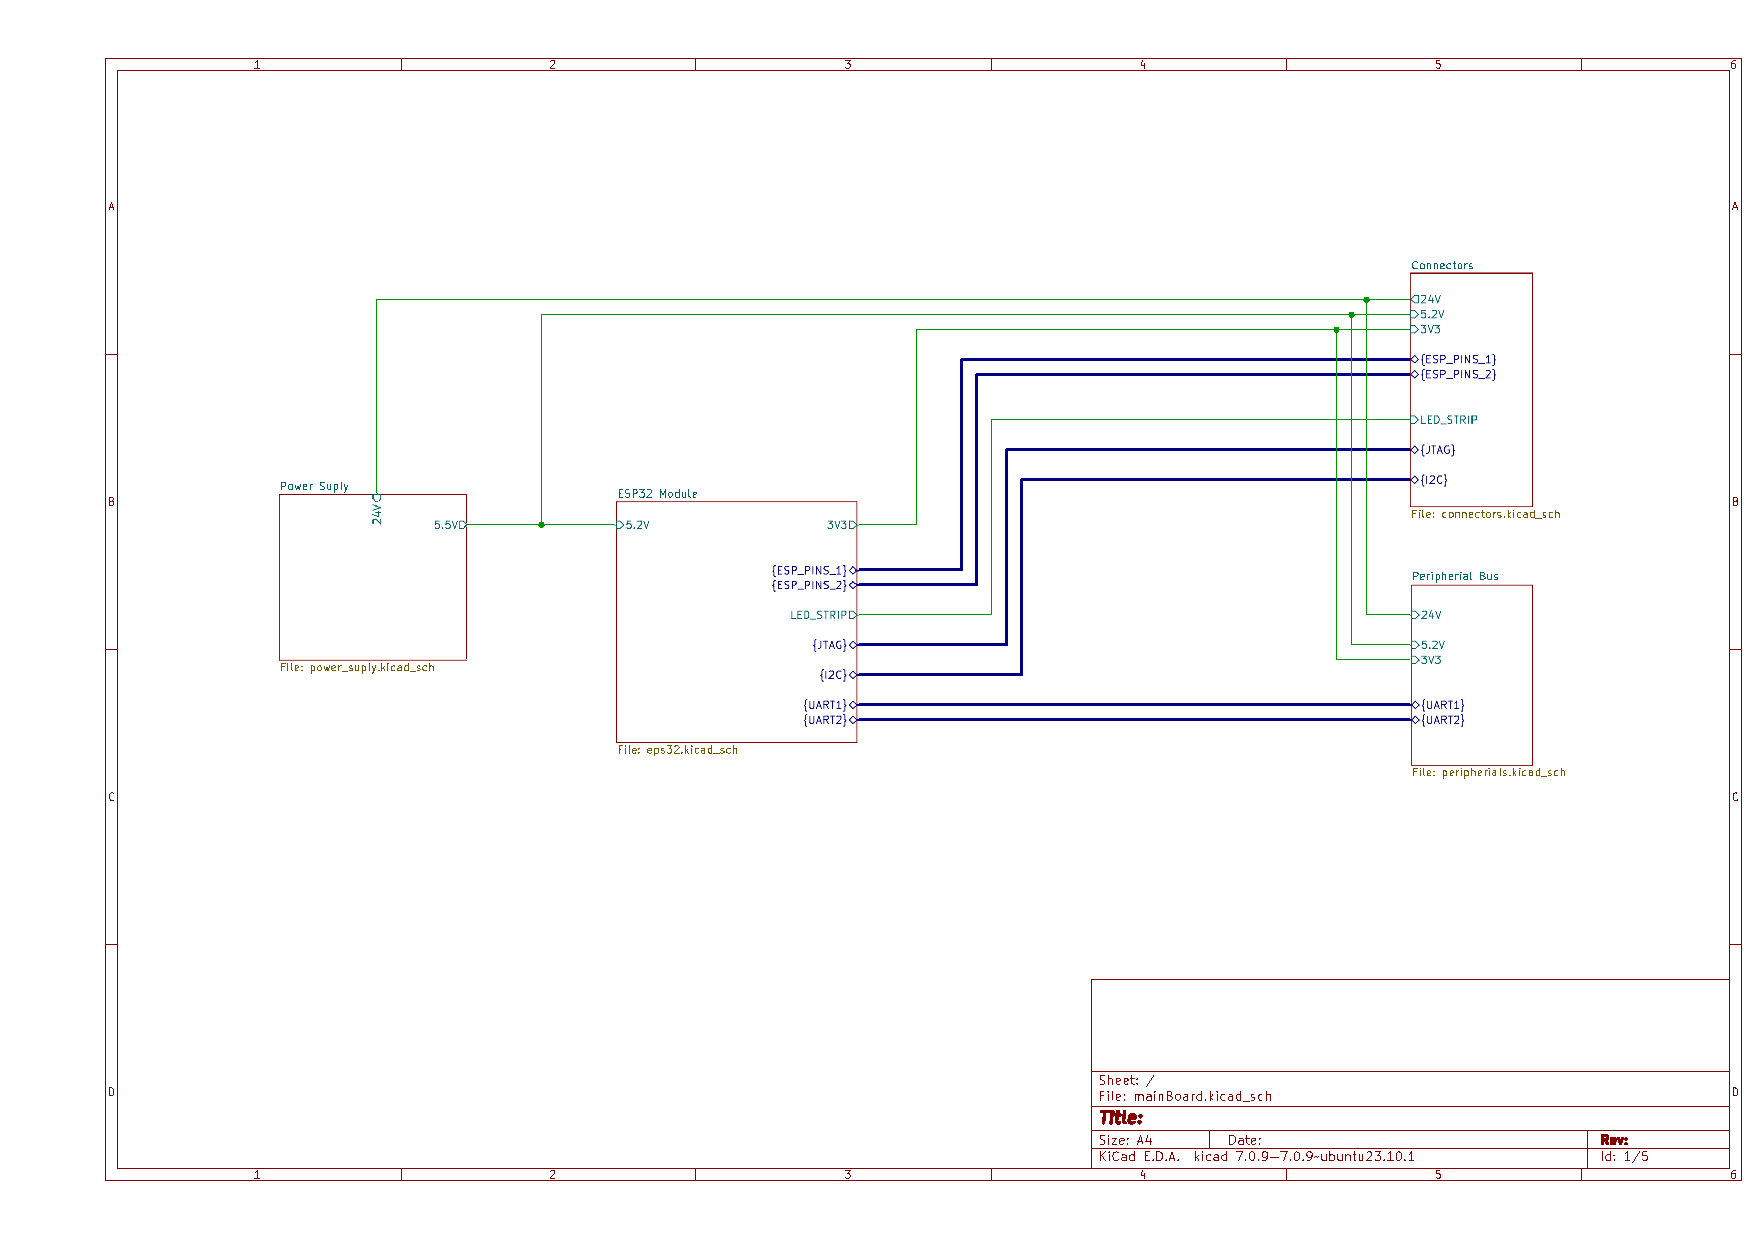
\includegraphics
	[
		width=\textheight, height=0.9\textwidth, keepaspectratio,
		page=1, 
		angle=90,
		trim=1.5cm 1cm 0cm 1cm, 
		clip
	]{obrazky/exportovane/main-board-schematic.pdf}

	\section{Zapojení MCU}
\label{priloha:schema-ridici-jednotka-mcu}
	% trim=left bottom right top
	\includegraphics
	[
		width=\textheight, height=\textwidth, keepaspectratio,
		page=2, 
		angle=90,
		trim=1.5cm 1cm 0cm 1cm, 
		clip
	]{obrazky/exportovane/main-board-schematic.pdf}

	\section{Napájecí obvod}
\label{priloha:schema-ridici-jednotka-napajeci-obvod}
	% trim=left bottom right top
	\includegraphics
	[
		width=\textheight, height=\textwidth, keepaspectratio,
		page=3, 
		angle=90,
		trim=1.5cm 1cm 0cm 1cm, 
		clip
	]{obrazky/exportovane/main-board-schematic.pdf}

	\section{Konektory}
\label{priloha:schema-ridici-jednotka-konektory}
	% trim=left bottom right top
	\includegraphics
	[
		width=\textheight, height=\textwidth, keepaspectratio,
		page=4, 
		angle=90,
		trim=1.5cm 1cm 0cm 1cm, 
		clip
	]{obrazky/exportovane/main-board-schematic.pdf}

	\section{Sběrnice periferií}
	\label{priloha:schema-ridici-jednotka-periferie}
		% trim=left bottom right top
		\includegraphics
		[
			width=\textheight, height=\textwidth, keepaspectratio,
			page=5, 
			angle=90,
			trim=1.5cm 1cm 0cm 1cm, 
			clip
		]{obrazky/exportovane/main-board-schematic.pdf}


\chapter{Schéma modulu periferií}
\label{priloha:schema-modul-periferii}
	% trim=left bottom right top
	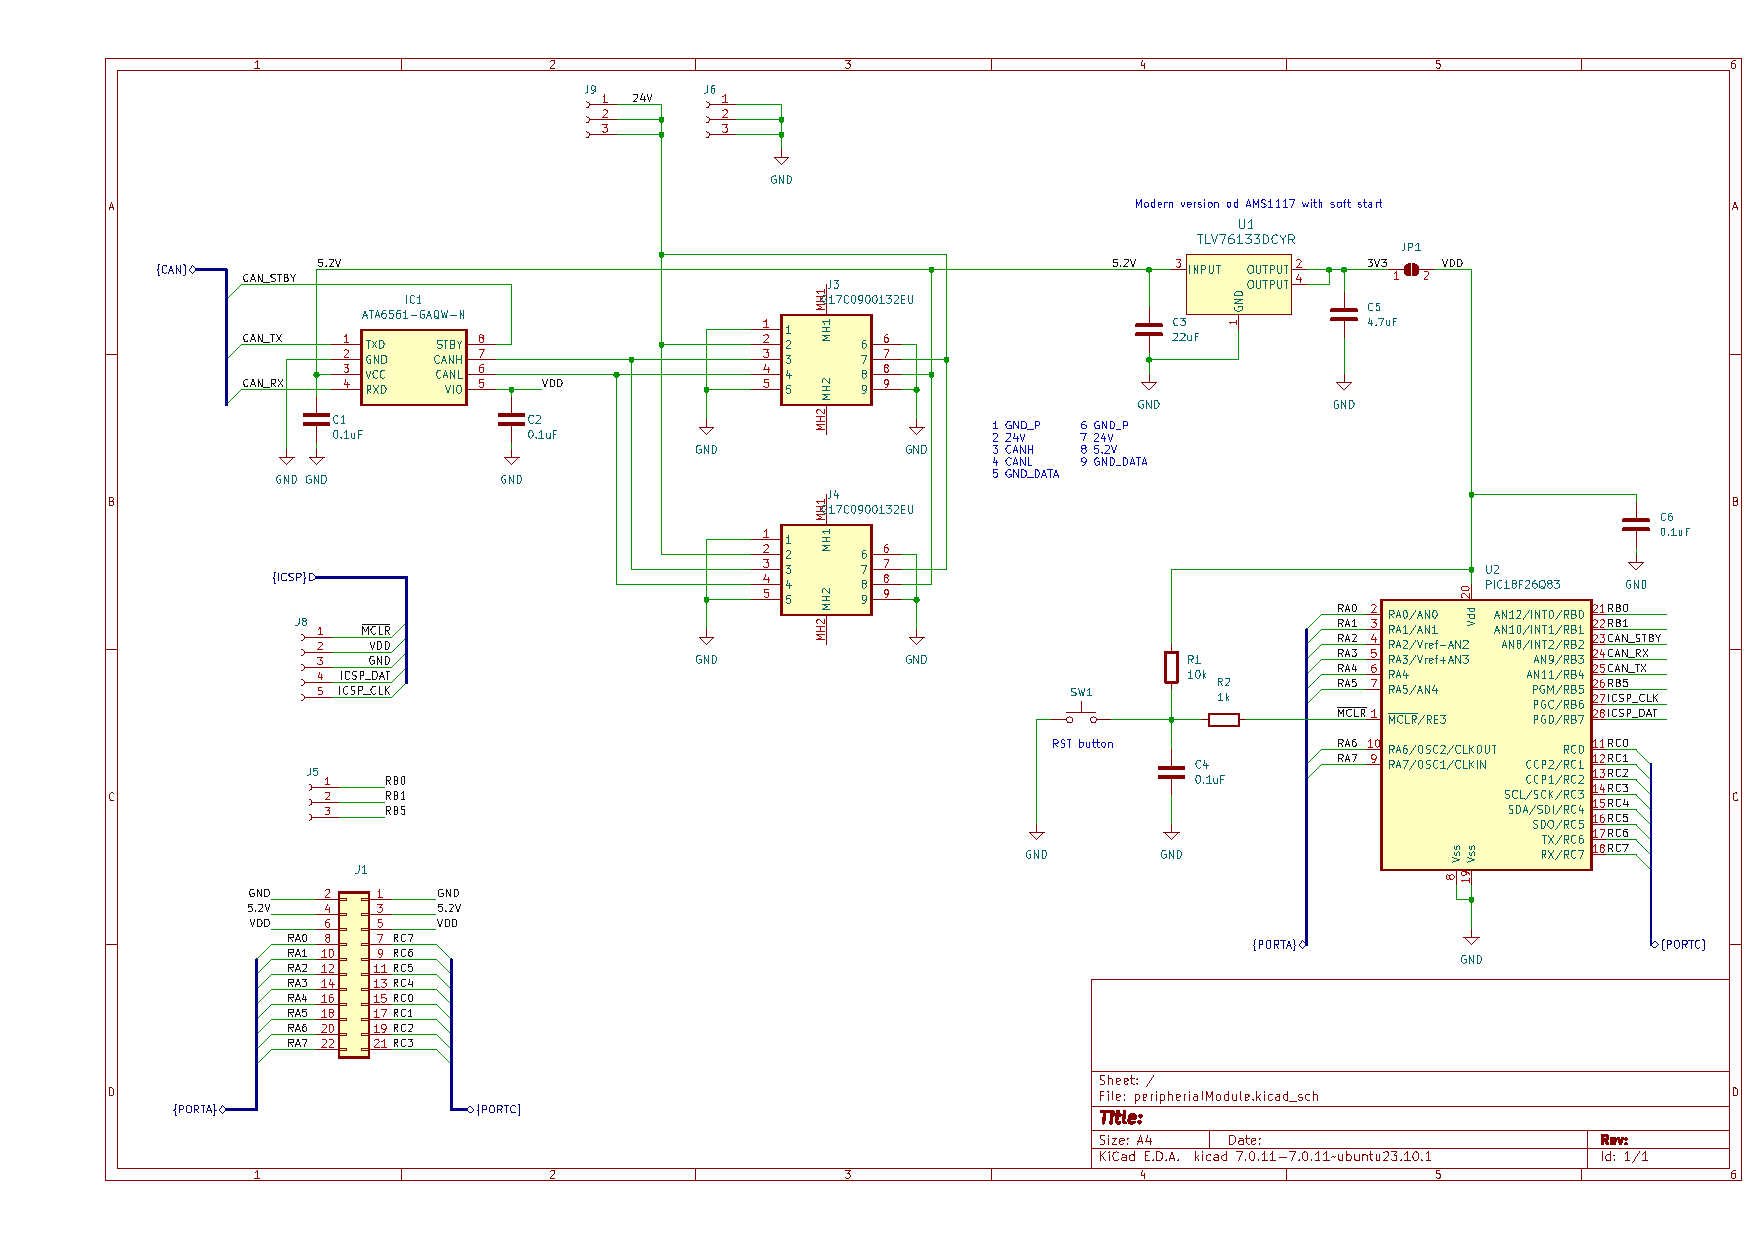
\includegraphics
	[
		width=\textheight, height=\textwidth, keepaspectratio,
		page=1, 
		angle=90,
		trim=1.5cm 1cm 0cm 1cm, 
		clip
	]{obrazky/exportovane/peripherial-module-schematic.pdf}

\chapter{Schéma modulu LED osvětlení}
\label{priloha:schema-led-board}
	% trim=left bottom right top
	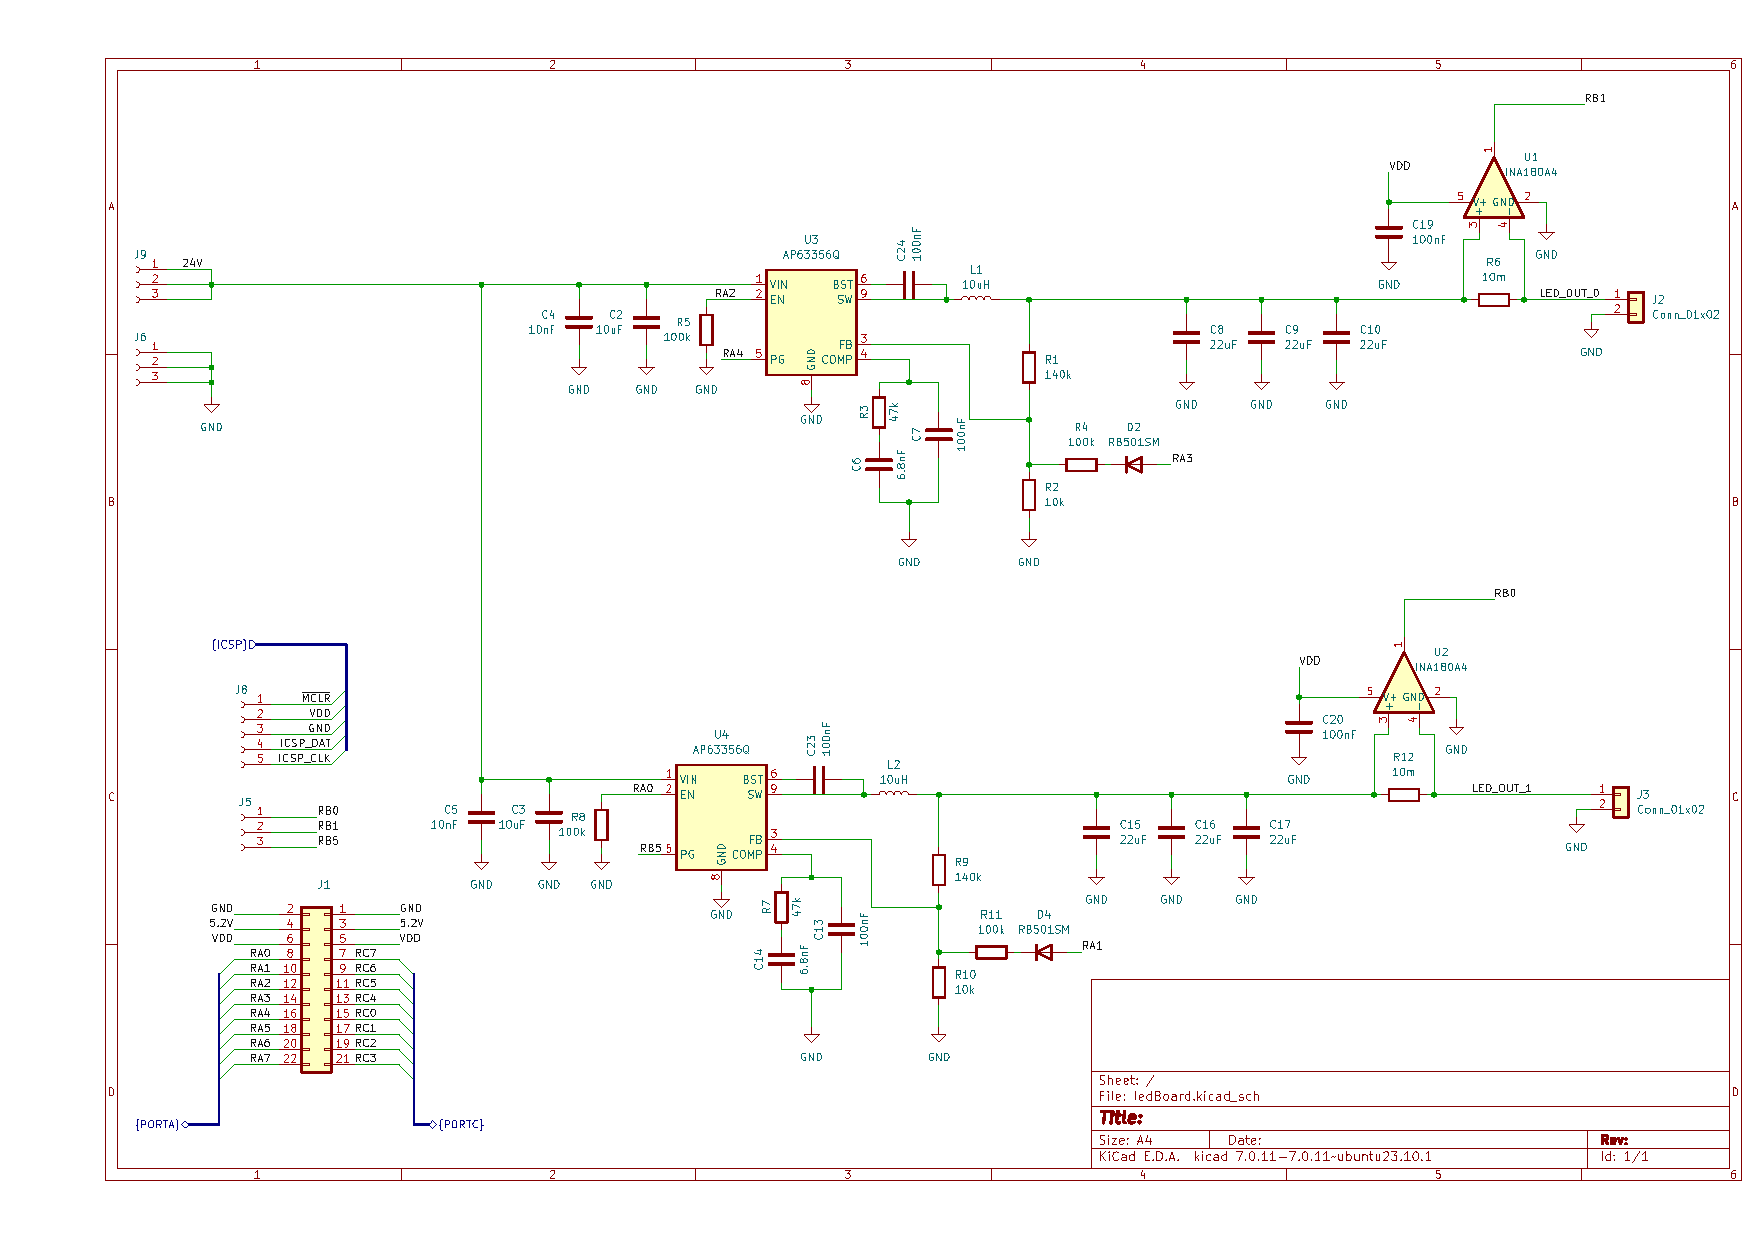
\includegraphics
	[
		width=\textheight, height=\textwidth, keepaspectratio,
		page=1, 
		angle=90,
		trim=1.5cm 1cm 0cm 1cm, 
		clip
	]{obrazky/exportovane/led-board-schematic.pdf}

\end{document}